\documentclass[xetex,mathserif,serif]{beamer}
\usepackage{polyglossia}
\setdefaultlanguage[babelshorthands=true]{russian}
\usepackage{minted}
\usepackage{tabu}

\useoutertheme{infolines}

\usepackage{fontspec}
\setmainfont{FreeSans}
\newfontfamily{\russianfonttt}{FreeSans}

\usepackage{textpos}
\setlength{\TPHorizModule}{1cm}
\setlength{\TPVertModule}{1cm}

\setbeamertemplate{blocks}[rounded][shadow=false]

\setbeamercolor*{block title alerted}{fg=red!50!black,bg=red!20}
\setbeamercolor*{block body alerted}{fg=black,bg=red!10}

\definecolor{links}{HTML}{2A1B81}
\hypersetup{colorlinks,linkcolor=,urlcolor=links}

\tabulinesep=1.2mm

\title[Моделирование]{Лекция 3: Моделирование, UML}
\author[Юрий Литвинов]{Юрий Литвинов\\\small{\textcolor{gray}{yurii.litvinov@gmail.com}}}
\date{21.09.2018г}

\newcommand{\todo}[1] {
	\begin{center}\textcolor{red}{TODO: #1}\end{center}
}

\newcommand{\DownArrow} {
	\hspace{2cm}\begin{LARGE}$\downarrow$\end{LARGE}
}

\newcommand{\attribution}[1] {
	\vspace{-5mm}\begin{flushright}\begin{scriptsize}\textcolor{gray}{\textcopyright\, #1}\end{scriptsize}\end{flushright}
}

\begin{document}

	\frame{\titlepage}

	\section{Модели}

	\begin{frame}
		\frametitle{Моделирование}
		\begin{itemize}
			\item \textbf{Модель} --- упрощённое подобие объекта или явления
			\item Нужны для изучения некоторых их свойств, абстрагируясь от сложности ``настоящего'' объекта или явления
			\item Модели используются повсеместно
			\begin{itemize}
				\item Математические модели
				\item Модели как реальные объекты
				\item Модели в разработке ПО
			\end{itemize}
		\end{itemize}
	\end{frame}

	\begin{frame}
		\frametitle{Общие свойства моделей}
		\begin{itemize}
			\item Содержат меньше информации, чем реальность
			\item Существуют для определённой цели
			\item Модели субъективны, что позволяет отделить существенные свойства от несущественных
			\item Модели ограничены
		\end{itemize}

		\center{\textbf{All models are wrong, some are useful}}
	\end{frame}

	\begin{frame}
		\frametitle{Моделирование ПО}
		\begin{itemize}
			\item Предназначены прежде всего для управления сложностью
			\item Могут моделировать как саму систему, так и окружение
			\item Позволяют понять, проанализировать и протестировать систему до её реализации
		\end{itemize}
		\begin{center}
			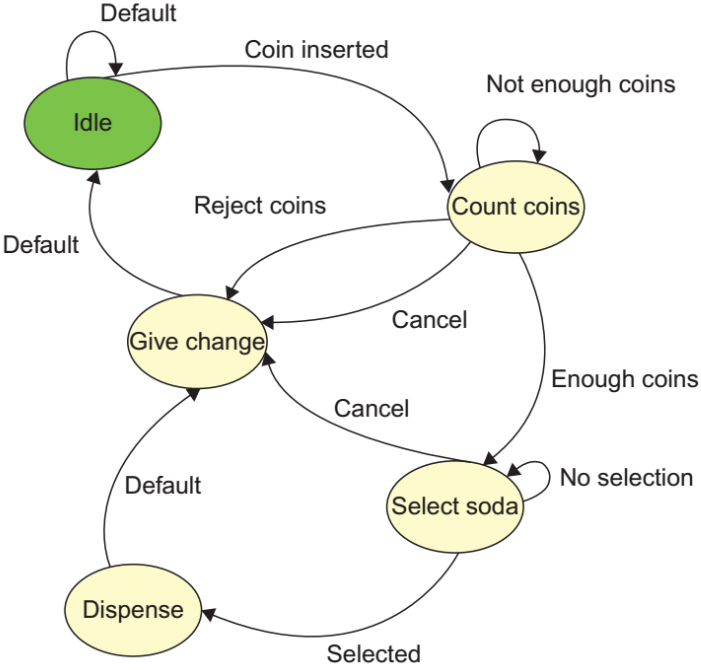
\includegraphics[width=0.4\textwidth]{vendingMachine.png}
			\attribution{N. Medvidovic}
		\end{center}
	\end{frame}

	\begin{frame}
		\frametitle{Модели бывают разные}
		\begin{itemize}
			\item Используемые нотации и способы моделирования зависят от целей моделирования
			\begin{itemize}
				\item От неформальных набросков до исполнимых моделей
			\end{itemize}
		\end{itemize}
		\begin{center}
			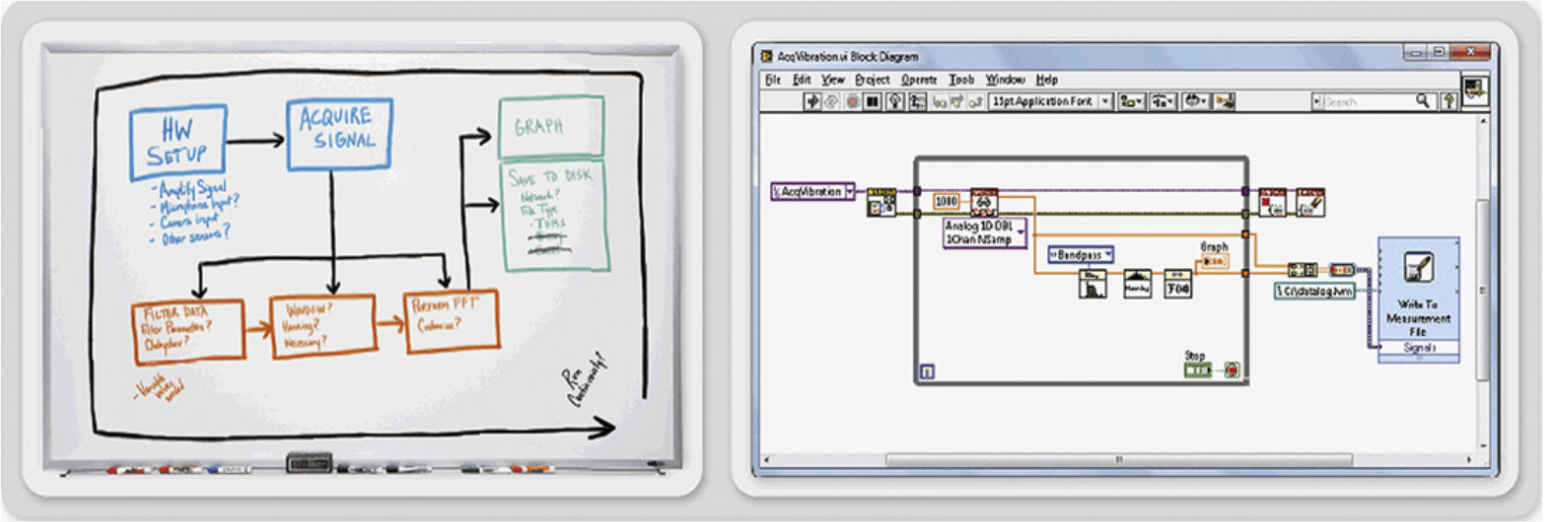
\includegraphics[width=0.9\textwidth]{sketchesVsFormalNotations.png}
			\attribution{N. Medvidovic}
		\end{center}
	\end{frame}

	\begin{frame}
		\frametitle{Архитектурные модели}
		\begin{itemize}
			\item Архитектура --- это набор основных решений, принятых для данной системы
			\item Архитектурная модель --- это некоторый артефакт, который отражает некоторые или все эти решения
			\item Архитектурное моделирование --- это процесс уточнения и документирования этих решений
			\item Моделирование непосредственно связано с используемой нотацией
			\begin{itemize}
				\item Нотация архитектурного моделирования --- это язык или другое средство описания архитектурных решений
			\end{itemize}
		\end{itemize}
	\end{frame}

	\begin{frame}
		\frametitle{Как выбрать, что моделировать?}
		\begin{itemize}
			\item При моделировании надо определиться с:
			\begin{itemize}
				\item Какие архитектурные решения нуждаются в моделировании
				\item На каком уровне детализации
				\item Насколько формально
			\end{itemize}
			\item Необходимо учитывать соотношение трудозатрат и выгоды
			\begin{itemize}
				\item Стоимость создания \textit{и поддержания} модели не должна быть больше преимуществ от её использования
			\end{itemize}
		\end{itemize}
		\begin{center}
			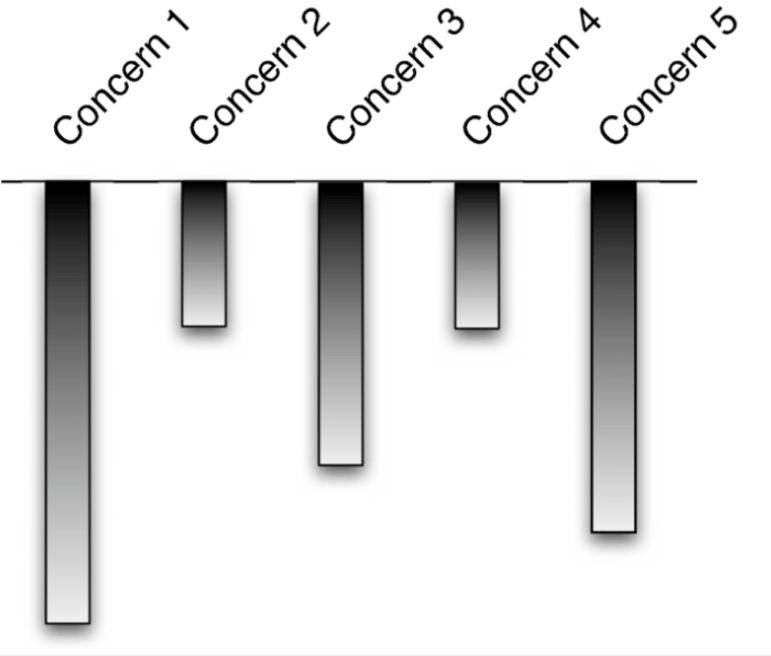
\includegraphics[width=0.4\textwidth]{concerns.png}
			\attribution{N. Medvidovic}
		\end{center}
	\end{frame}

	\begin{frame}
		\frametitle{Возможные преимущества моделей}
		\begin{itemize}
			\item Инструмент, направляющий и облегчающий проектирование
			\item Средство коммуникации между разработчиками
			\item Наглядный инструмент для общения с заказчиком
			\item Средство документирования и фиксации принятых решений
			\item Исходник для генерации кода?
		\end{itemize}
		\begin{center}
			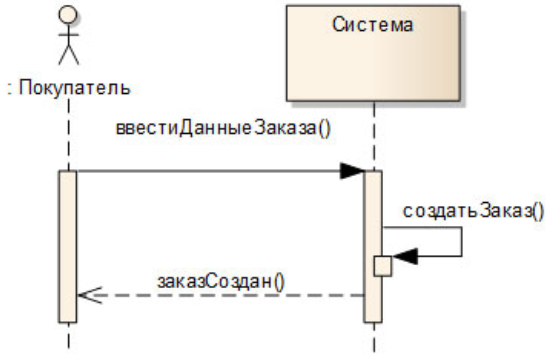
\includegraphics[width=0.4\textwidth]{sequenceDiagram.png}
		\end{center}
	\end{frame}

	\section{Виды моделей}

	\begin{frame}
		\frametitle{Виды моделей}
		\framesubtitle{Естественные языки}
		\begin{columns}
			\begin{column}{0.5\textwidth}
				\begin{itemize}
					\item Обычный текст --- вполне себе инструмент моделирования
					\item Очень выразителен, не требует специальных знаний, максимально гибок
					\item Неоднозначен, неформален, не строг, слишком многословен, бесполезен для автоматической обработки
				\end{itemize}
			\end{column}
			\begin{column}{0.5\textwidth}
				\begin{center}
					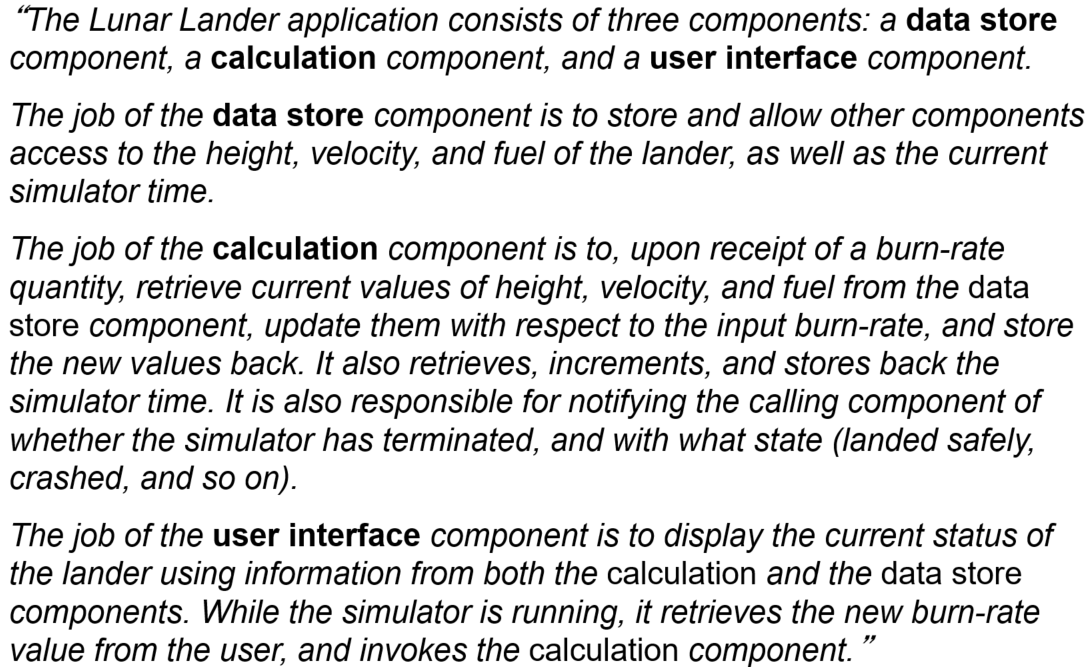
\includegraphics[width=\textwidth]{naturalLanguage.png}
					\attribution{N. Medvidovic}
				\end{center}
			\end{column}
		\end{columns}
	\end{frame}

	\begin{frame}
		\frametitle{Неформальные графические модели}
		\begin{columns}
			\begin{column}{0.5\textwidth}
				\begin{itemize}
					\item Диаграммы, рисуемые в PowerPoint, InkScape и подобном
					\item Могут быть красивыми, как правило, простые, очень гибкая нотация
					\item Неформальны, неоднозначны, не строги
					\begin{itemize}
						\item Но часто воспринимаются наоборот
					\end{itemize}
					\item Практически бесполезны для автоматической обработки
				\end{itemize}
			\end{column}
			\begin{column}{0.5\textwidth}
				\begin{center}
					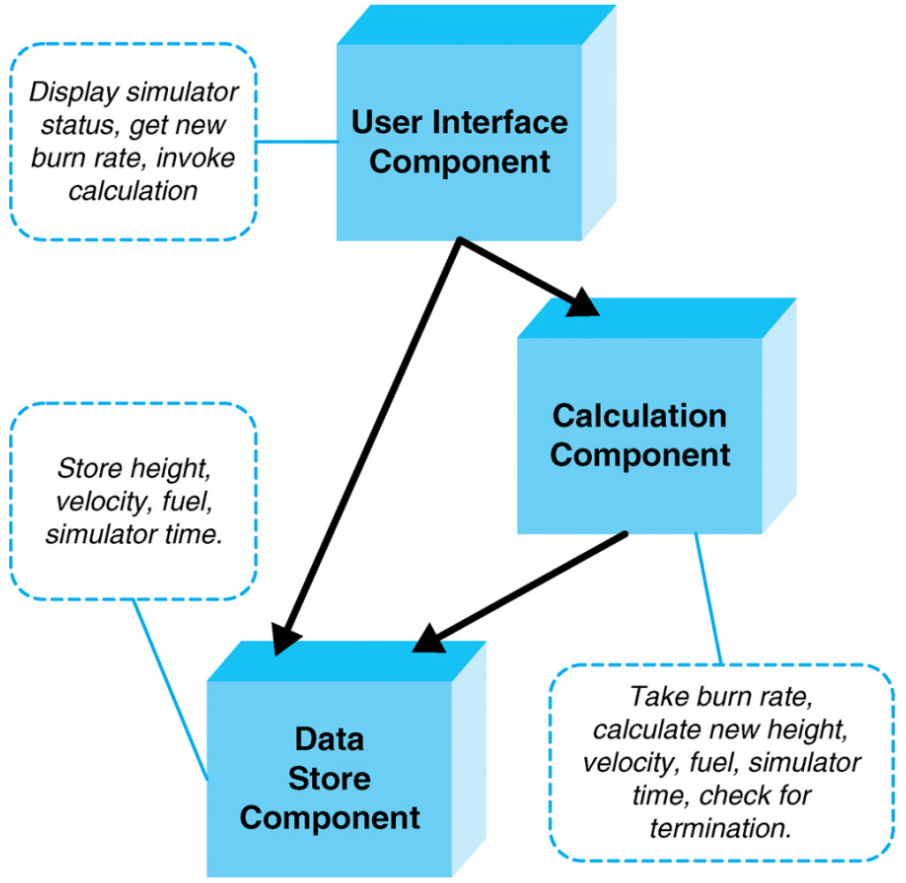
\includegraphics[width=0.9\textwidth]{informalModel.png}
					\attribution{N. Medvidovic}
				\end{center}
			\end{column}
		\end{columns}
	\end{frame}

	\begin{frame}
		\frametitle{UML и SysML}
		\begin{columns}
			\begin{column}{0.4\textwidth}
				\begin{small}
					\begin{itemize}
						\item Несколько слабо связанных нотаций (``диаграмм'')
						\item Поддерживают много точек зрения, общеприняты, широкая поддержка инструментами
						\item Нет строгой семантики, сложно обеспечить консистентность, сложно расширять
					\end{itemize}
				\end{small}
			\end{column}
			\begin{column}{0.6\textwidth}
				\begin{center}
					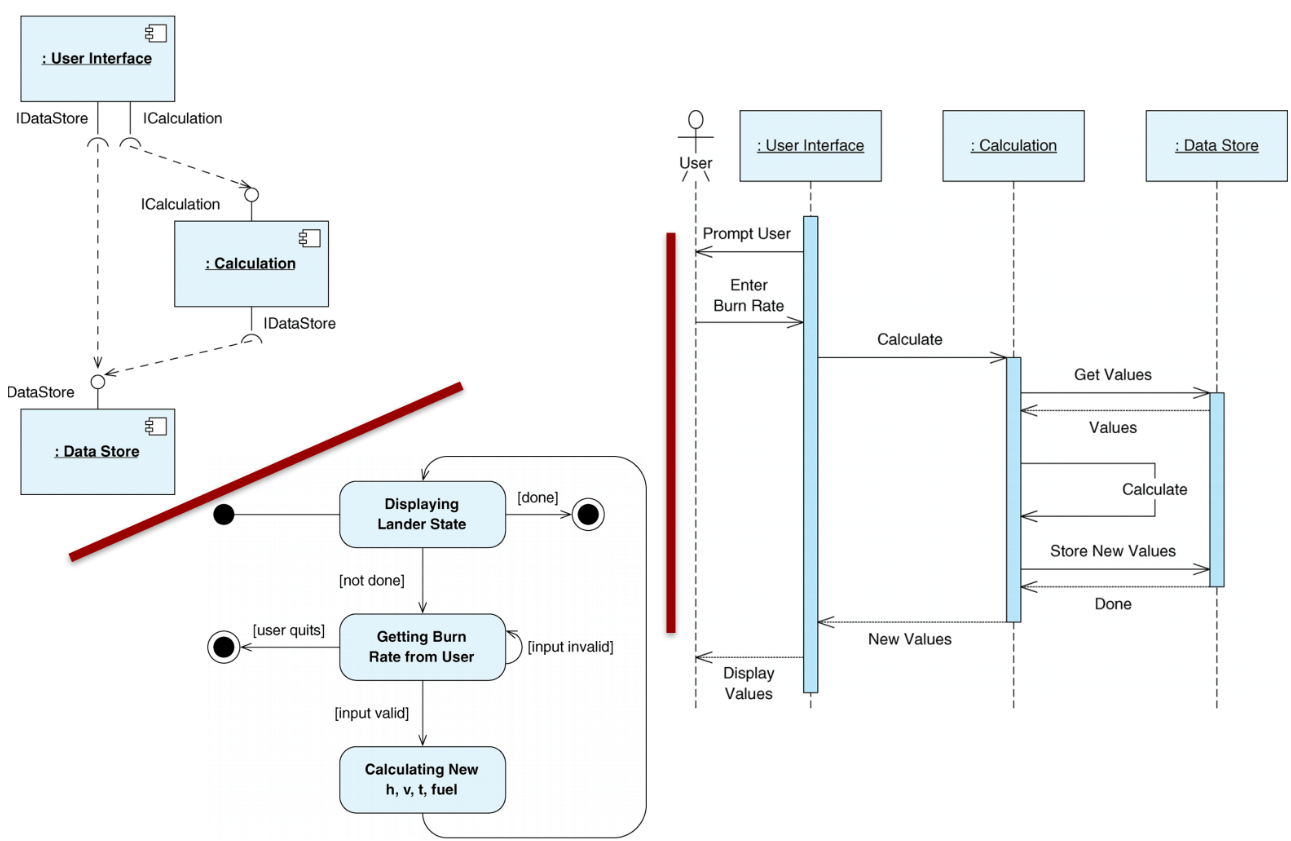
\includegraphics[width=\textwidth]{uml.png}
					\attribution{N. Medvidovic}
				\end{center}
			\end{column}
		\end{columns}
	\end{frame}

	\begin{frame}
		\frametitle{AADL и другие текстовые формальные языки}
		\begin{columns}
			\begin{column}{0.4\textwidth}
				\begin{small}
					\begin{itemize}
						\item Хороши для моделирования встроенных систем и систем реального времени
						\item Описывают одновременно ``железо'' и ``софт'', продвинутые инструменты анализа
						\item Слишком многословны и детальны, сложны в изучении и использовании
					\end{itemize}
				\end{small}
			\end{column}
			\begin{column}{0.6\textwidth}
				\begin{center}
					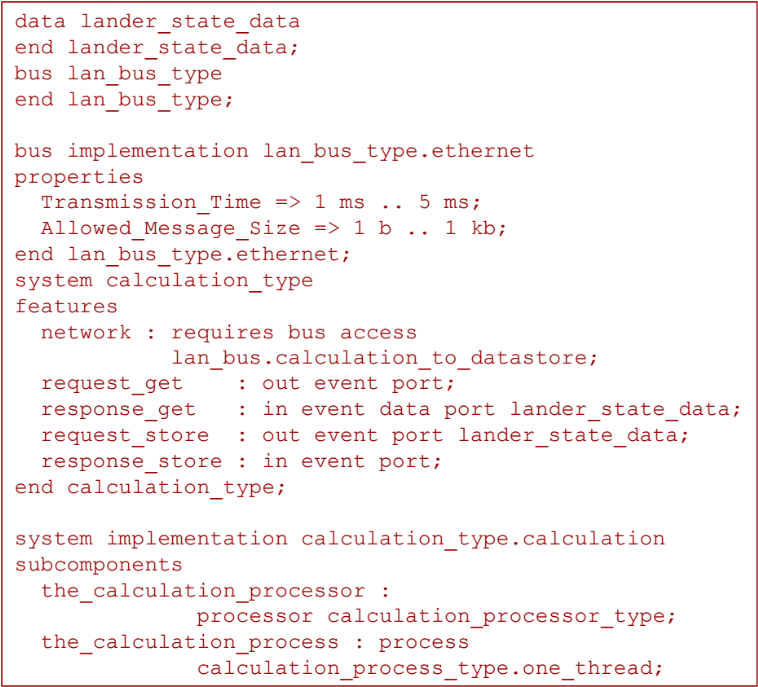
\includegraphics[width=0.85\textwidth]{aadl.png}
					\attribution{N. Medvidovic}
				\end{center}
			\end{column}
		\end{columns}
	\end{frame}

	\section{UML}

	\begin{frame}
		\frametitle{Вернёмся к визуальным моделям}
		\begin{itemize}
			\item \textbf{Метафора визуализации} --- договорённость о том, как будут представляться сущности языка
			\item \textbf{Точка зрения моделирования} --- какой аспект системы и для кого моделируется
			\item Бывают одноразовые модели, документация и графические исходники
			\begin{itemize}
				\item \textbf{Семантический разрыв} --- неспособность модели полностью специфицировать систему
			\end{itemize}
		\end{itemize}
		\begin{center}
			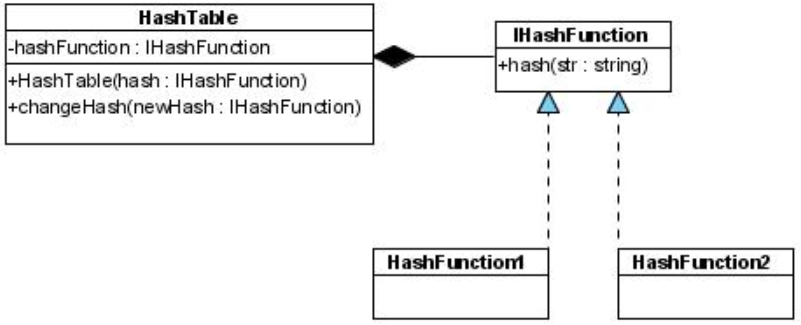
\includegraphics[width=0.5\textwidth]{hashTable.png}
		\end{center}
	\end{frame}

	\begin{frame}
		\frametitle{Unified Modeling Language}
		\begin{itemize}
			\item Семейство графических нотаций
			\begin{itemize}
				\item 14 видов диаграмм
			\end{itemize}
			\item Общая метамодель
			\item Стандарт под управлением Object Management Group
			\begin{itemize}
				\item UML 1.1 --- 1997 год
				\item UML 2.0 --- 2005 год
				\item UML 2.5.1 --- декабрь 2017 года
			\end{itemize}
			\item Прежде всего, для проектирования ПО
			\begin{itemize}
				\item После UML 2.0 стали появляться нотации и для инженеров
			\end{itemize}
			\item Расширяем
			\begin{itemize}
				\item Профили --- механизм легковесного расширения
				\item Метамоделирование
			\end{itemize}
		\end{itemize}
	\end{frame}

	\begin{frame}
		\frametitle{История}
		\begin{center}
			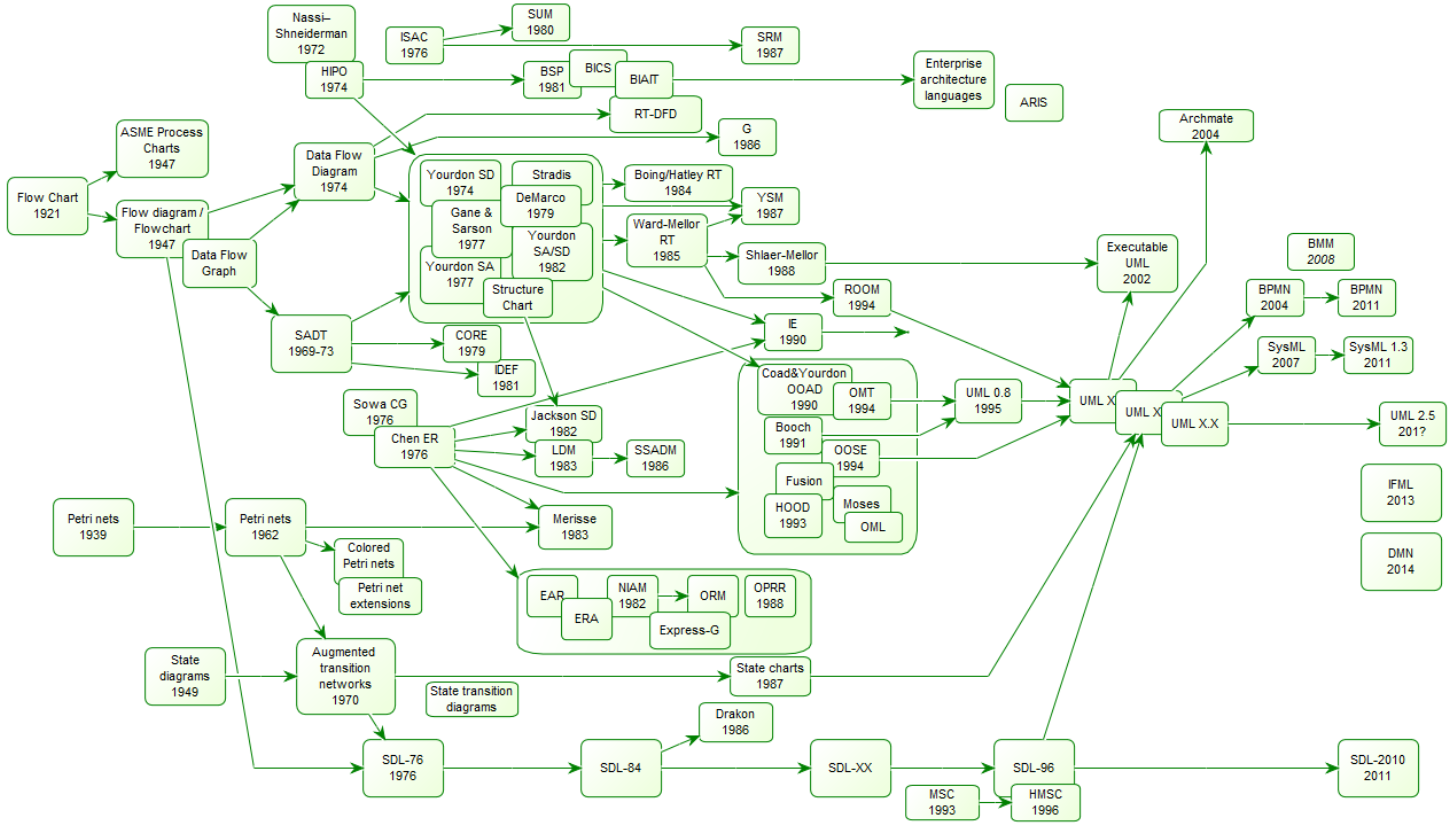
\includegraphics[width=\textwidth]{umlHistory.png}
		\end{center}
	\end{frame}

	\begin{frame}
		\frametitle{Виды диаграмм}
		\begin{center}
			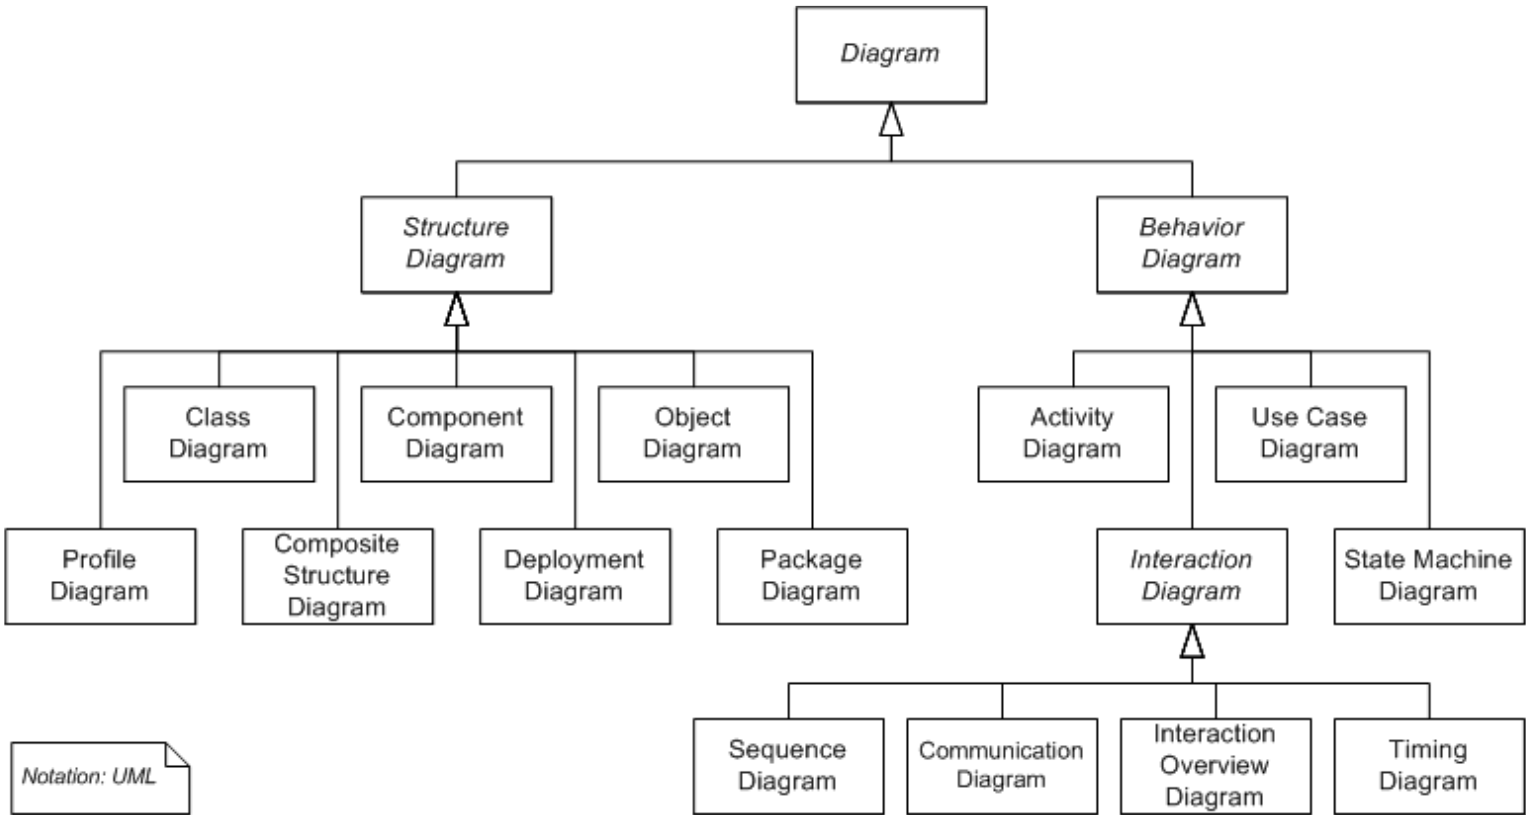
\includegraphics[width=\textwidth]{umlDiagrams.png}
		\end{center}
	\end{frame}

	\section{Диаграмма классов UML}

	\begin{frame}
		\frametitle{Диаграмма классов}
		\begin{center}
			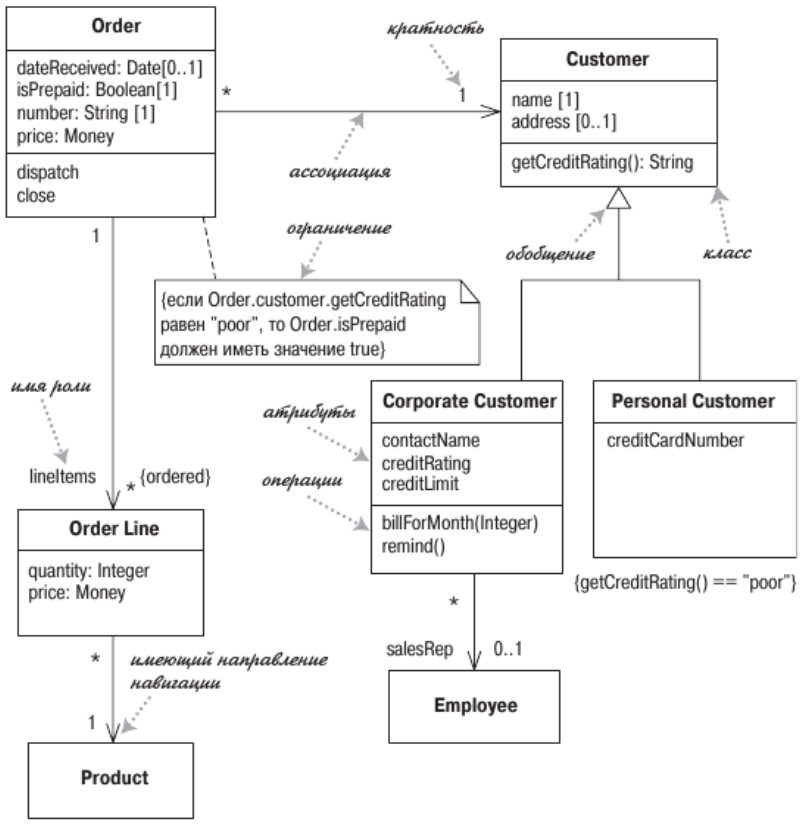
\includegraphics[height=0.8\textheight]{umlClassDiagram.png}
			\attribution{М. Фаулер. ``UML. Основы''}
		\end{center}
	\end{frame}

	\begin{frame}
		\frametitle{Свойства}
		\begin{columns}
			\begin{column}{0.5\textwidth}
				Атрибуты:
				\begin{center}
					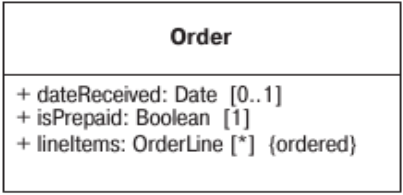
\includegraphics[width=0.5\textwidth]{attributes.png}
				\end{center}
			\end{column}
			\begin{column}{0.5\textwidth}
				Ассоциация-класс:
				\begin{center}
					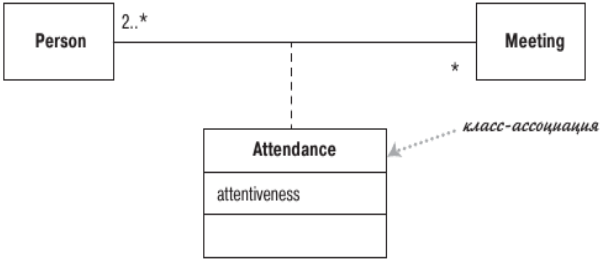
\includegraphics[width=0.85\textwidth]{classAssociation.png}
				\end{center}
			\end{column}
		\end{columns}
		\vspace{5mm}
		Ассоциации:
		\begin{center}
			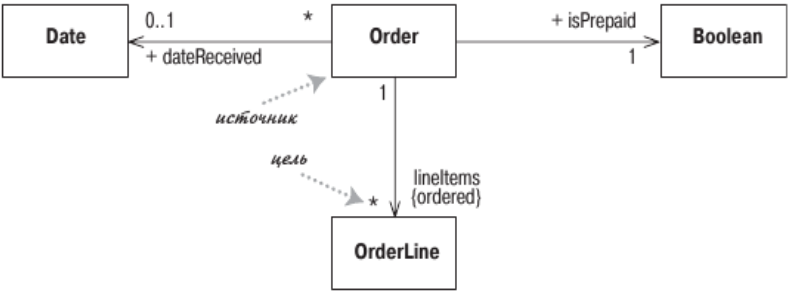
\includegraphics[width=0.5\textwidth]{associations.png}
		\end{center}
		\attribution{М. Фаулер. ``UML. Основы''}
	\end{frame}

	\begin{frame}
		\frametitle{Синтаксис свойств}
		\begin{itemize}
			\item Объявление поля:
			\begin{itemize}
				\item \texttt{видимость имя: тип кратность = значение по умолчанию \{строка свойств\}}
			\end{itemize}
			\item Видимость:
			\begin{itemize}
				\item \texttt{$+$ (public), $-$ (private), \# (protected), \textasciitilde (package)}
			\end{itemize}
			\item Кратность:
			\begin{itemize}
				\item \texttt{1} (ровно 1 объект), \texttt{0..1} (ни одного или один), \texttt{*} (сколько угодно), \texttt{1..*}, \texttt{2..*}
			\end{itemize}
		\end{itemize}
	\end{frame}

	\begin{frame}[fragile]
		\frametitle{Как это связано с кодом}
		\begin{columns}
			\begin{column}{0.5\textwidth}
				\begin{footnotesize}
					\begin{minted}{java}
public class OrderLine {
    private int quantity;
    private Product product;
    public int getQuantity() {
        return quantity;
    }
    public void setQuantity(int quantity) {
        this.quantity = quantity;
    }
    public Money getPrice() {
        return product.getPrice().multiply(quantity);
    }
}
					\end{minted}
				\end{footnotesize}
			\end{column}
			\begin{column}{0.5\textwidth}
				\begin{center}
					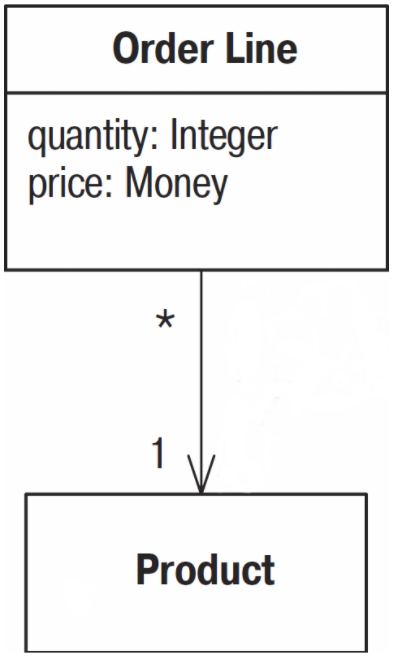
\includegraphics[width=0.5\textwidth]{orderLine.png}
				\end{center}
			\end{column}
		\end{columns}
	\end{frame}

	\begin{frame}[fragile]
		\frametitle{Двунаправленные ассоциации}
		\begin{columns}
			\begin{column}{0.5\textwidth}
				\begin{scriptsize}
					\begin{center}
						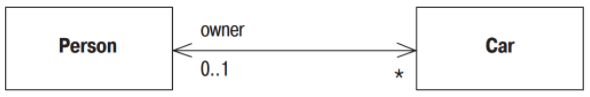
\includegraphics[width=0.9\textwidth]{twoWayAssociations.png}
					\end{center}
	
					\begin{minted}{csharp}
class Car {
    public Person Owner {
        get { return _owner; }
        set {
            if (_owner != null) 
                _owner.friendCars().Remove(this);
            _owner = value;
            if (_owner != null) 
                _owner.friendCars().Add(this);
        }
    }
    private Person _owner;
}
					\end{minted}
				\end{scriptsize}
				\vspace{2mm}
			\end{column}
			\begin{column}{0.5\textwidth}
				\begin{scriptsize}
					\begin{center}
						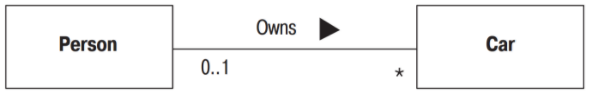
\includegraphics[width=0.9\textwidth]{personOwnsCar.png}
					\end{center}
	
					\begin{minted}{csharp}
class Person {
    public IList Cars {
        get { return ArrayList.ReadOnly(_cars); }
    }
    public void AddCar(Car arg) {
        arg.Owner = this;
    }
    private IList _cars = new ArrayList();
    internal IList friendCars() {
        // должен быть использован 
        // только Car.Owner
        return _cars;
    }
}
					\end{minted}
				\end{scriptsize}
			\end{column}
		\end{columns}
	\end{frame}

	\begin{frame}
		\frametitle{Интерфейсы}
		\begin{center}
			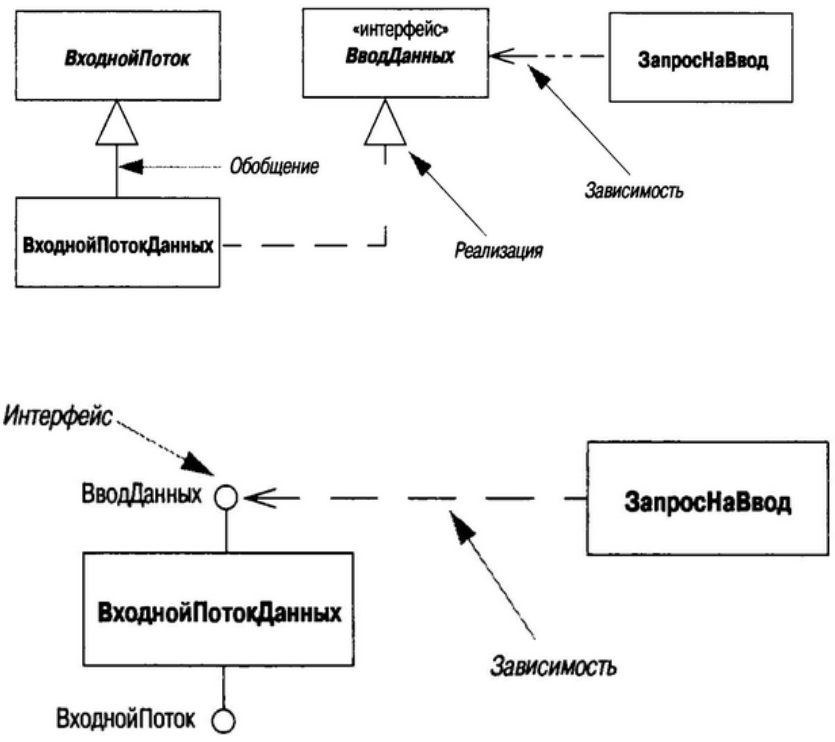
\includegraphics[width=0.6\textwidth]{interfaces.png}
			\attribution{М. Фаулер. ``UML. Основы''}
		\end{center}
	\end{frame}

	\begin{frame}
		\frametitle{Зависимости}
		\begin{columns}
			\begin{column}{0.3\textwidth}
				\begin{itemize}
					\item call
					\item create
					\item derive
					\item permit 
				\end{itemize}
			\end{column}
			\begin{column}{0.3\textwidth}
				\begin{itemize}
					\item realize
					\item substitute
					\item instantiate
					\item refine 
				\end{itemize}
			\end{column}
			\begin{column}{0.3\textwidth}
				\begin{itemize}
					\item trace
					\item use
					\item ...
				\end{itemize}
			\end{column}
		\end{columns}
		\vspace{7mm}
		\begin{center}
			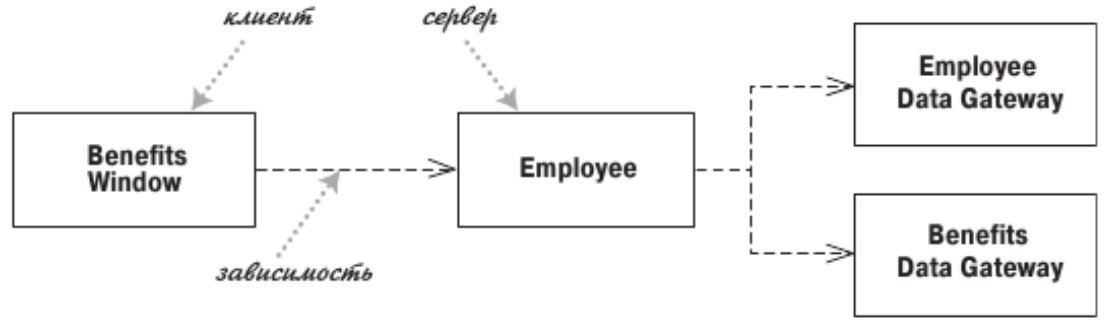
\includegraphics[width=0.5\textwidth]{dependencies.png}
			\attribution{М. Фаулер. ``UML. Основы''}
		\end{center}
	\end{frame}

	\begin{frame}
		\frametitle{Агрегация и композиция}
		Агрегация:
		\begin{center}
			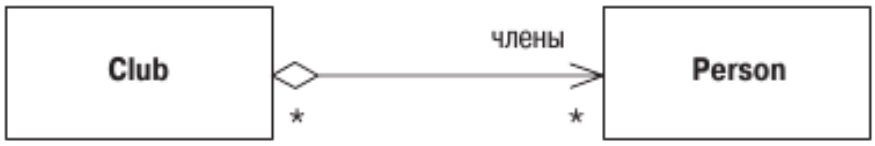
\includegraphics[height=0.1\textheight]{aggregation.png}
		\end{center}
		\vspace{5mm}
		Композиция:
		\begin{center}
			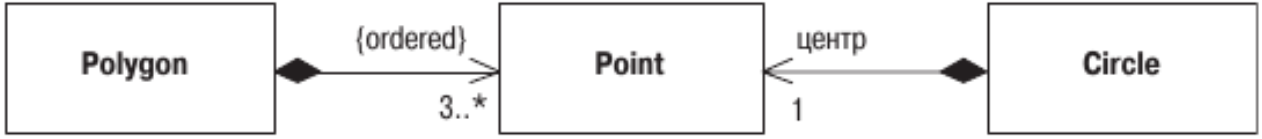
\includegraphics[height=0.1\textheight]{composition.png}
		\end{center}
		\attribution{М. Фаулер. ``UML. Основы''}
	\end{frame}

	\begin{frame}
		\frametitle{Агрегация и композиция, пример}
		\begin{center}
			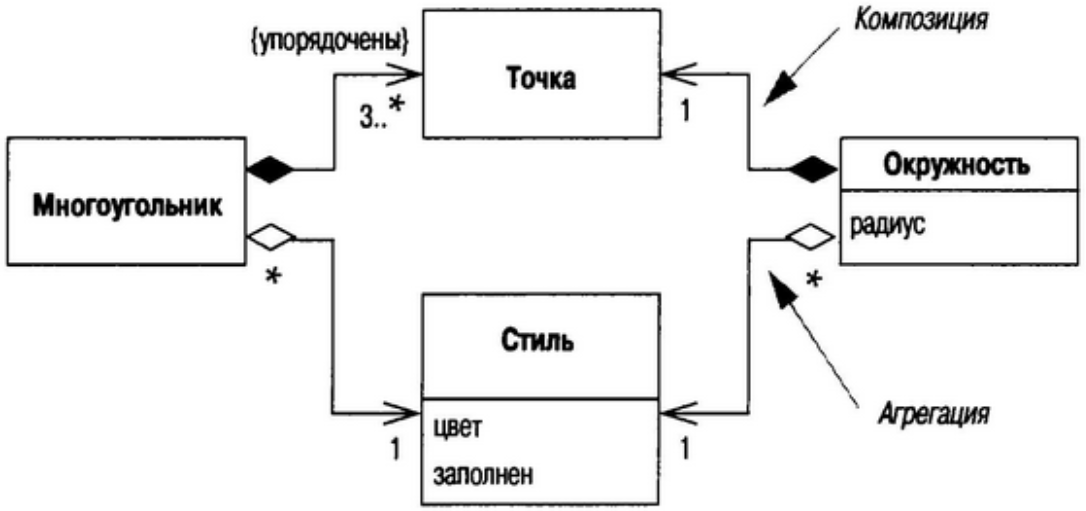
\includegraphics[width=0.7\textwidth]{aggregationAndCompositionExample.png}
			\attribution{М. Фаулер. ``UML. Основы''}
		\end{center}
	\end{frame}

	\begin{frame}
		\frametitle{Шаблоны и перечисления}
		\begin{center}
			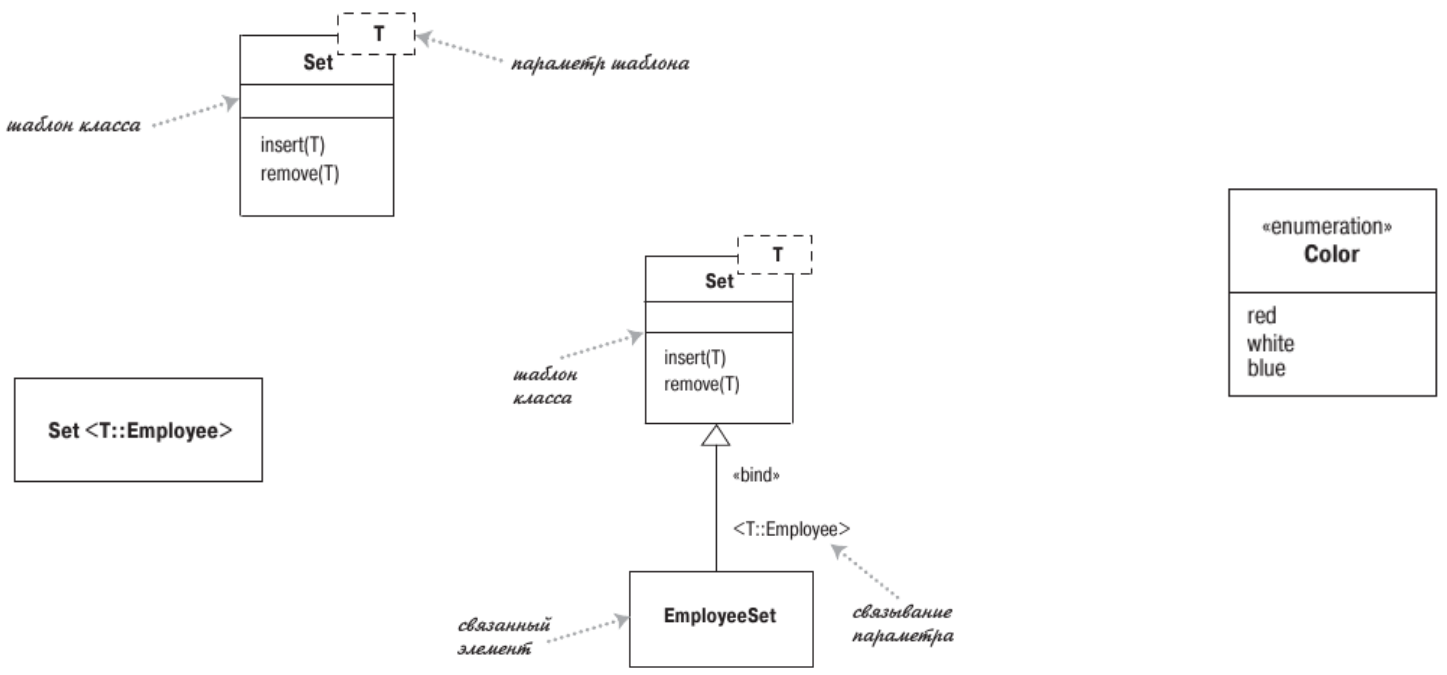
\includegraphics[width=0.95\textwidth]{genericsAndEnums.png}
			\attribution{М. Фаулер. ``UML. Основы''}
		\end{center}
	\end{frame}

	\section{Диаграммы пакетов}

	\begin{frame}
		\frametitle{Диаграммы пакетов}
		\begin{center}
			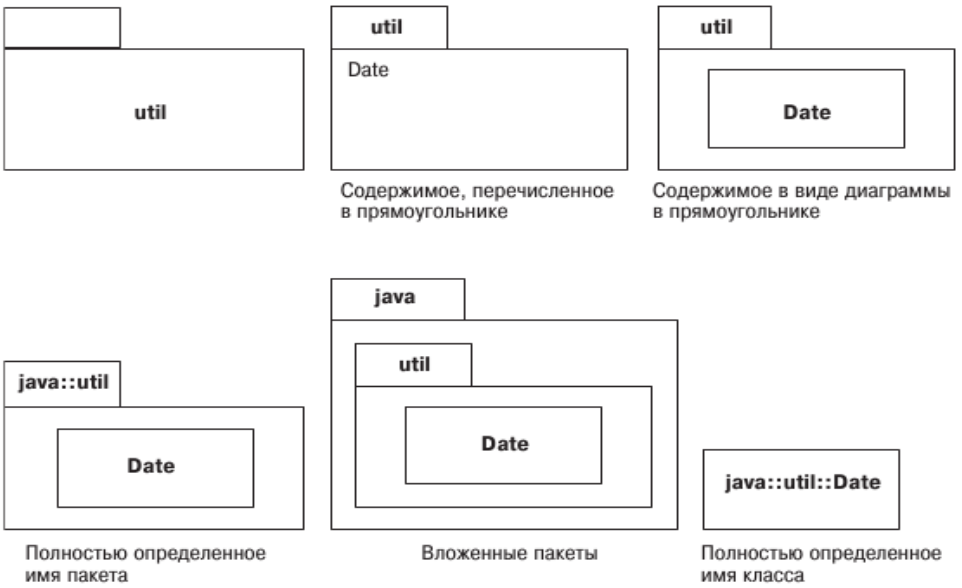
\includegraphics[width=0.8\textwidth]{packageDiagrams.png}
			\attribution{М. Фаулер. ``UML. Основы''}
		\end{center}
	\end{frame}

	\begin{frame}
		\frametitle{Диаграммы пакетов, зависимости}
		\begin{center}
			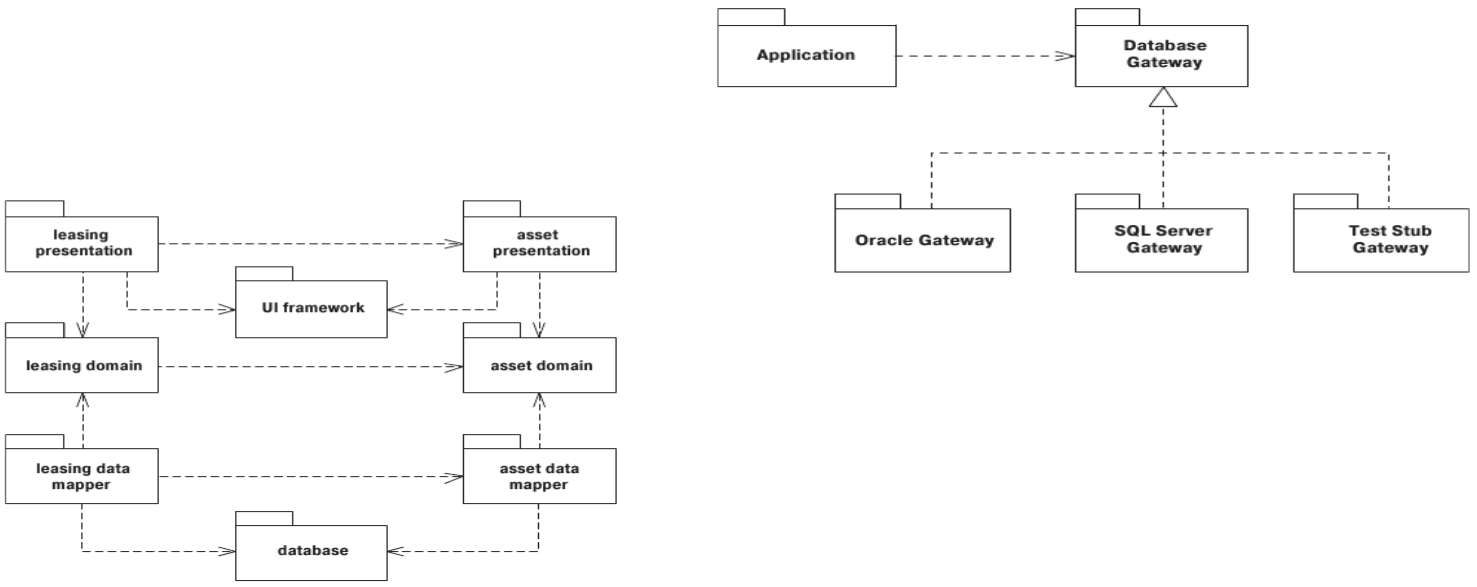
\includegraphics[width=0.95\textwidth]{packageDependencies.png}
			\attribution{М. Фаулер. ``UML. Основы''}
		\end{center}
	\end{frame}

	\section{Диаграммы объектов}

	\begin{frame}
		\frametitle{Диаграммы объектов}
		\begin{center}
			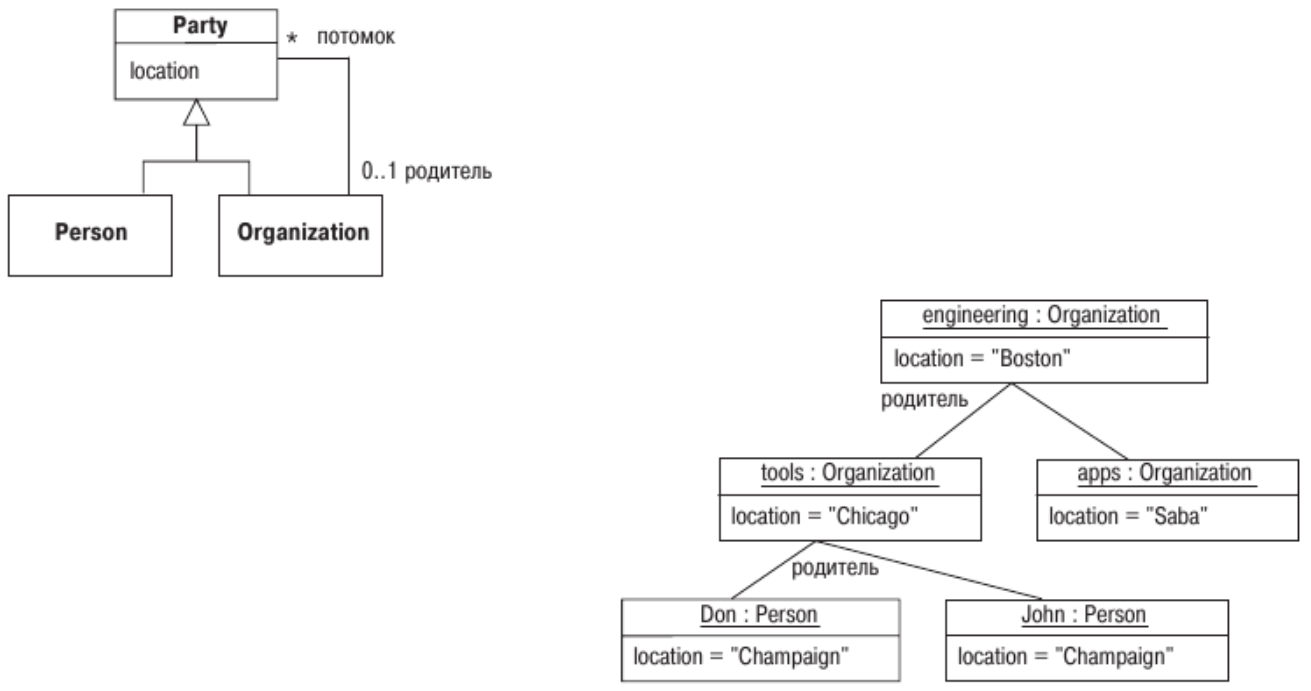
\includegraphics[width=0.9\textwidth]{objectDiagrams.png}
			\attribution{М. Фаулер. ``UML. Основы''}
		\end{center}
	\end{frame}

	\section{Диаграммы компонентов}
	
	\begin{frame}
		\frametitle{Диаграммы компонентов}
		\begin{center}
			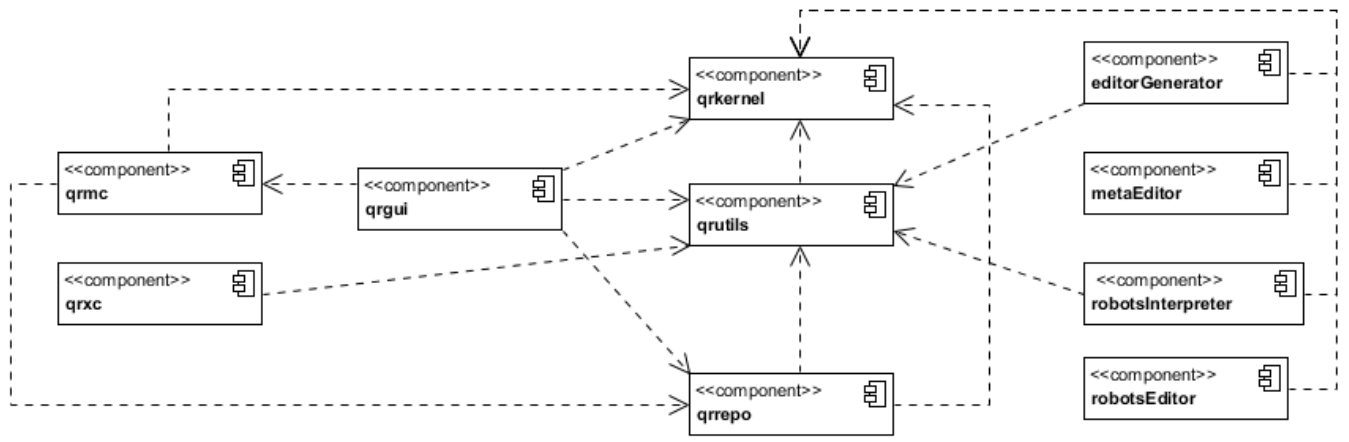
\includegraphics[width=0.95\textwidth]{componentDiagrams.png}
		\end{center}
	\end{frame}

	\begin{frame}
		\frametitle{Более подробно}
		\begin{center}
			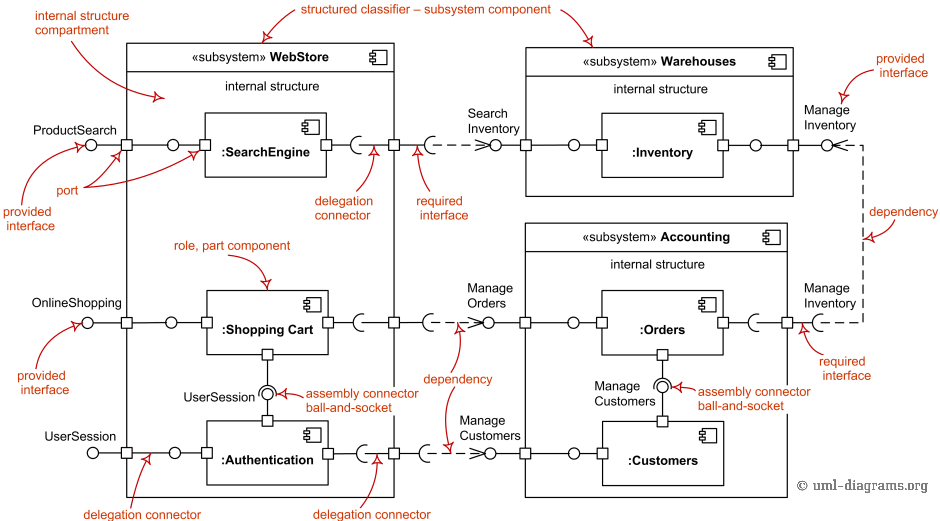
\includegraphics[width=0.95\textwidth]{componentDiagramsOverview.png}
			\attribution{\url{http://www.uml-diagrams.org}}
		\end{center}
	\end{frame}

\end{document}
